\documentclass[1p]{elsarticle_modified}
%\bibliographystyle{elsarticle-num}

%\usepackage[colorlinks]{hyperref}
%\usepackage{abbrmath_seonhwa} %\Abb, \Ascr, \Acal ,\Abf, \Afrak
\usepackage{amsfonts}
\usepackage{amssymb}
\usepackage{amsmath}
\usepackage{amsthm}
\usepackage{scalefnt}
\usepackage{amsbsy}
\usepackage{kotex}
\usepackage{caption}
\usepackage{subfig}
\usepackage{color}
\usepackage{graphicx}
\usepackage{xcolor} %% white, black, red, green, blue, cyan, magenta, yellow
\usepackage{float}
\usepackage{setspace}
\usepackage{hyperref}

\usepackage{tikz}
\usetikzlibrary{arrows}

\usepackage{multirow}
\usepackage{array} % fixed length table
\usepackage{hhline}

%%%%%%%%%%%%%%%%%%%%%
\makeatletter
\renewcommand*\env@matrix[1][\arraystretch]{%
	\edef\arraystretch{#1}%
	\hskip -\arraycolsep
	\let\@ifnextchar\new@ifnextchar
	\array{*\c@MaxMatrixCols c}}
\makeatother %https://tex.stackexchange.com/questions/14071/how-can-i-increase-the-line-spacing-in-a-matrix
%%%%%%%%%%%%%%%

\usepackage[normalem]{ulem}

\newcommand{\msout}[1]{\ifmmode\text{\sout{\ensuremath{#1}}}\else\sout{#1}\fi}
%SOURCE: \msout is \stkout macro in https://tex.stackexchange.com/questions/20609/strikeout-in-math-mode

\newcommand{\cancel}[1]{
	\ifmmode
	{\color{red}\msout{#1}}
	\else
	{\color{red}\sout{#1}}
	\fi
}

\newcommand{\add}[1]{
	{\color{blue}\uwave{#1}}
}

\newcommand{\replace}[2]{
	\ifmmode
	{\color{red}\msout{#1}}{\color{blue}\uwave{#2}}
	\else
	{\color{red}\sout{#1}}{\color{blue}\uwave{#2}}
	\fi
}

\newcommand{\Sol}{\mathcal{S}} %segment
\newcommand{\D}{D} %diagram
\newcommand{\A}{\mathcal{A}} %arc


%%%%%%%%%%%%%%%%%%%%%%%%%%%%%5 test

\def\sl{\operatorname{\textup{SL}}(2,\Cbb)}
\def\psl{\operatorname{\textup{PSL}}(2,\Cbb)}
\def\quan{\mkern 1mu \triangleright \mkern 1mu}

\theoremstyle{definition}
\newtheorem{thm}{Theorem}[section]
\newtheorem{prop}[thm]{Proposition}
\newtheorem{lem}[thm]{Lemma}
\newtheorem{ques}[thm]{Question}
\newtheorem{cor}[thm]{Corollary}
\newtheorem{defn}[thm]{Definition}
\newtheorem{exam}[thm]{Example}
\newtheorem{rmk}[thm]{Remark}
\newtheorem{alg}[thm]{Algorithm}

\newcommand{\I}{\sqrt{-1}}
\begin{document}

%\begin{frontmatter}
%
%\title{Boundary parabolic representations of knots up to 8 crossings}
%
%%% Group authors per affiliation:
%\author{Yunhi Cho} 
%\address{Department of Mathematics, University of Seoul, Seoul, Korea}
%\ead{yhcho@uos.ac.kr}
%
%
%\author{Seonhwa Kim} %\fnref{s_kim}}
%\address{Center for Geometry and Physics, Institute for Basic Science, Pohang, 37673, Korea}
%\ead{ryeona17@ibs.re.kr}
%
%\author{Hyuk Kim}
%\address{Department of Mathematical Sciences, Seoul National University, Seoul 08826, Korea}
%\ead{hyukkim@snu.ac.kr}
%
%\author{Seokbeom Yoon}
%\address{Department of Mathematical Sciences, Seoul National University, Seoul, 08826,  Korea}
%\ead{sbyoon15@snu.ac.kr}
%
%\begin{abstract}
%We find all boundary parabolic representation of knots up to 8 crossings.
%
%\end{abstract}
%\begin{keyword}
%    \MSC[2010] 57M25 
%\end{keyword}
%
%\end{frontmatter}

%\linenumbers
%\tableofcontents
%
\newcommand\colored[1]{\textcolor{white}{\rule[-0.35ex]{0.8em}{1.4ex}}\kern-0.8em\color{red} #1}%
%\newcommand\colored[1]{\textcolor{white}{ #1}\kern-2.17ex	\textcolor{white}{ #1}\kern-1.81ex	\textcolor{white}{ #1}\kern-2.15ex\color{red}#1	}

{\Large $\underline{12a_{0812}~(K12a_{0812})}$}

\setlength{\tabcolsep}{10pt}
\renewcommand{\arraystretch}{1.6}
\vspace{1cm}\begin{tabular}{m{100pt}>{\centering\arraybackslash}m{274pt}}
\multirow{5}{120pt}{
	\centering
	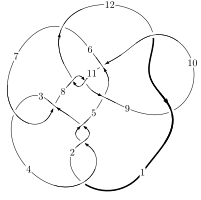
\includegraphics[width=112pt]{../../../GIT/diagram.site/Diagrams/png/1613_12a_0812.png}\\
\ \ \ A knot diagram\footnotemark}&
\allowdisplaybreaks
\textbf{Linearized knot diagam} \\
\cline{2-2}
 &
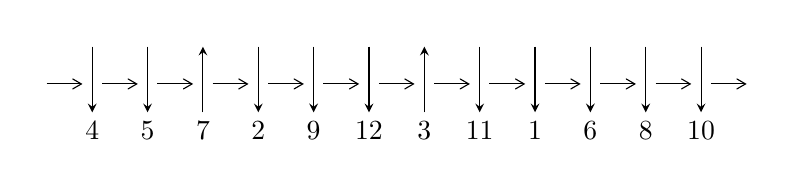
\begin{tikzpicture}[x=20pt, y=17pt]
	% nodes
	\node (C0) at (0, 0) {};
	\node (C1) at (1, 0) {};
	\node (C1U) at (1, +1) {};
	\node (C1D) at (1, -1) {4};

	\node (C2) at (2, 0) {};
	\node (C2U) at (2, +1) {};
	\node (C2D) at (2, -1) {5};

	\node (C3) at (3, 0) {};
	\node (C3U) at (3, +1) {};
	\node (C3D) at (3, -1) {7};

	\node (C4) at (4, 0) {};
	\node (C4U) at (4, +1) {};
	\node (C4D) at (4, -1) {2};

	\node (C5) at (5, 0) {};
	\node (C5U) at (5, +1) {};
	\node (C5D) at (5, -1) {9};

	\node (C6) at (6, 0) {};
	\node (C6U) at (6, +1) {};
	\node (C6D) at (6, -1) {12};

	\node (C7) at (7, 0) {};
	\node (C7U) at (7, +1) {};
	\node (C7D) at (7, -1) {3};

	\node (C8) at (8, 0) {};
	\node (C8U) at (8, +1) {};
	\node (C8D) at (8, -1) {11};

	\node (C9) at (9, 0) {};
	\node (C9U) at (9, +1) {};
	\node (C9D) at (9, -1) {1};

	\node (C10) at (10, 0) {};
	\node (C10U) at (10, +1) {};
	\node (C10D) at (10, -1) {6};

	\node (C11) at (11, 0) {};
	\node (C11U) at (11, +1) {};
	\node (C11D) at (11, -1) {8};

	\node (C12) at (12, 0) {};
	\node (C12U) at (12, +1) {};
	\node (C12D) at (12, -1) {10};
	\node (C13) at (13, 0) {};

	% arrows
	\draw[->,>={angle 60}]
	(C0) edge (C1) (C1) edge (C2) (C2) edge (C3) (C3) edge (C4) (C4) edge (C5) (C5) edge (C6) (C6) edge (C7) (C7) edge (C8) (C8) edge (C9) (C9) edge (C10) (C10) edge (C11) (C11) edge (C12) (C12) edge (C13) ;	\draw[->,>=stealth]
	(C1U) edge (C1D) (C2U) edge (C2D) (C3D) edge (C3U) (C4U) edge (C4D) (C5U) edge (C5D) (C6U) edge (C6D) (C7D) edge (C7U) (C8U) edge (C8D) (C9U) edge (C9D) (C10U) edge (C10D) (C11U) edge (C11D) (C12U) edge (C12D) ;
	\end{tikzpicture} \\
\hhline{~~} \\& 
\textbf{Solving Sequence} \\ \cline{2-2} 
 &
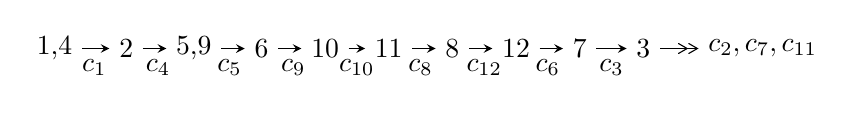
\begin{tikzpicture}[x=23pt, y=7pt]
	% node
	\node (A0) at (-1/8, 0) {1,4};
	\node (A1) at (1, 0) {2};
	\node (A2) at (33/16, 0) {5,9};
	\node (A3) at (25/8, 0) {6};
	\node (A4) at (33/8, 0) {10};
	\node (A5) at (41/8, 0) {11};
	\node (A6) at (49/8, 0) {8};
	\node (A7) at (57/8, 0) {12};
	\node (A8) at (65/8, 0) {7};
	\node (A9) at (73/8, 0) {3};
	\node (C1) at (1/2, -1) {$c_{1}$};
	\node (C2) at (3/2, -1) {$c_{4}$};
	\node (C3) at (21/8, -1) {$c_{5}$};
	\node (C4) at (29/8, -1) {$c_{9}$};
	\node (C5) at (37/8, -1) {$c_{10}$};
	\node (C6) at (45/8, -1) {$c_{8}$};
	\node (C7) at (53/8, -1) {$c_{12}$};
	\node (C8) at (61/8, -1) {$c_{6}$};
	\node (C9) at (69/8, -1) {$c_{3}$};
	\node (A10) at (11, 0) {$c_{2},c_{7},c_{11}$};

	% edge
	\draw[->,>=stealth]	
	(A0) edge (A1) (A1) edge (A2) (A2) edge (A3) (A3) edge (A4) (A4) edge (A5) (A5) edge (A6) (A6) edge (A7) (A7) edge (A8) (A8) edge (A9) ;
	\draw[->>,>={angle 60}]	
	(A9) edge (A10);
\end{tikzpicture} \\ 

\end{tabular} \\

\footnotetext{
The image of knot diagram is generated by the software ``\textbf{Draw programme}" developed by Andrew Bartholomew(\url{http://www.layer8.co.uk/maths/draw/index.htm\#Running-draw}), where we modified some parts for our purpose(\url{https://github.com/CATsTAILs/LinksPainter}).
}\phantom \\ \newline 
\centering \textbf{Ideals for irreducible components\footnotemark of $X_{\text{par}}$} 
 
\begin{align*}
I^u_{1}&=\langle 
1.08509\times10^{47} u^{41}+2.04550\times10^{47} u^{40}+\cdots+6.21177\times10^{47} b-1.86338\times10^{48},\\
\phantom{I^u_{1}}&\phantom{= \langle  }5.29448\times10^{46} u^{41}+1.94560\times10^{47} u^{40}+\cdots+2.48471\times10^{48} a-1.28814\times10^{49},\\
\phantom{I^u_{1}}&\phantom{= \langle  }u^{42}+3 u^{41}+\cdots-193 u-16\rangle \\
I^u_{2}&=\langle 
-19470 u^{34} a+16063 u^{34}+\cdots+14876 a-16265,\;5 u^{34} a-2 u^{34}+\cdots-3 a-42,\\
\phantom{I^u_{2}}&\phantom{= \langle  }u^{35}+3 u^{34}+\cdots+u-1\rangle \\
I^u_{3}&=\langle 
4 a^2+b-5 a+2,\;4 a^3-5 a^2+3 a-1,\;u-1\rangle \\
I^u_{4}&=\langle 
b+1,\;2 u^3+2 u^2+2 a-2 u+1,\;u^5+u^4-2 u^3- u^2+u-1\rangle \\
I^u_{5}&=\langle 
- a^3+3 a^2+b-5 a+2,\;a^4-3 a^3+5 a^2-3 a+1,\;u-1\rangle \\
\\
\end{align*}
\raggedright * 5 irreducible components of $\dim_{\mathbb{C}}=0$, with total 124 representations.\\
\footnotetext{All coefficients of polynomials are rational numbers. But the coefficients are sometimes approximated in decimal forms when there is not enough margin.}
\newpage
\renewcommand{\arraystretch}{1}
\centering \section*{I. $I^u_{1}= \langle 1.09\times10^{47} u^{41}+2.05\times10^{47} u^{40}+\cdots+6.21\times10^{47} b-1.86\times10^{48},\;5.29\times10^{46} u^{41}+1.95\times10^{47} u^{40}+\cdots+2.48\times10^{48} a-1.29\times10^{49},\;u^{42}+3 u^{41}+\cdots-193 u-16 \rangle$}
\flushleft \textbf{(i) Arc colorings}\\
\begin{tabular}{m{7pt} m{180pt} m{7pt} m{180pt} }
\flushright $a_{1}=$&$\begin{pmatrix}1\\0\end{pmatrix}$ \\
\flushright $a_{4}=$&$\begin{pmatrix}0\\u\end{pmatrix}$ \\
\flushright $a_{2}=$&$\begin{pmatrix}1\\u^2\end{pmatrix}$ \\
\flushright $a_{5}=$&$\begin{pmatrix}- u\\- u^3+u\end{pmatrix}$ \\
\flushright $a_{9}=$&$\begin{pmatrix}-0.0213082 u^{41}-0.0783029 u^{40}+\cdots-15.6524 u+5.18428\\-0.174683 u^{41}-0.329294 u^{40}+\cdots+27.4193 u+2.99976\end{pmatrix}$ \\
\flushright $a_{6}=$&$\begin{pmatrix}0.0226884 u^{41}+0.0558900 u^{40}+\cdots-11.7167 u+1.98961\\0.101268 u^{41}+0.188266 u^{40}+\cdots-17.0252 u-1.36379\end{pmatrix}$ \\
\flushright $a_{10}=$&$\begin{pmatrix}0.153375 u^{41}+0.250991 u^{40}+\cdots-43.0717 u+2.18452\\-0.174683 u^{41}-0.329294 u^{40}+\cdots+27.4193 u+2.99976\end{pmatrix}$ \\
\flushright $a_{11}=$&$\begin{pmatrix}0.0127553 u^{41}-0.0150214 u^{40}+\cdots-16.9996 u+2.86365\\0.0542267 u^{41}+0.114915 u^{40}+\cdots-8.87829 u-0.362657\end{pmatrix}$ \\
\flushright $a_{8}=$&$\begin{pmatrix}-0.0348739 u^{41}-0.0901865 u^{40}+\cdots-4.77020 u+3.86624\\0.483980 u^{41}+0.895391 u^{40}+\cdots-78.1740 u-6.66305\end{pmatrix}$ \\
\flushright $a_{12}=$&$\begin{pmatrix}0.0139183 u^{41}+0.0517931 u^{40}+\cdots+8.25026 u-1.43381\\-0.100313 u^{41}-0.210125 u^{40}+\cdots+16.6956 u+1.23646\end{pmatrix}$ \\
\flushright $a_{7}=$&$\begin{pmatrix}-0.0504330 u^{41}-0.0839435 u^{40}+\cdots+1.76064 u+4.15274\\0.481308 u^{41}+0.909837 u^{40}+\cdots-80.3209 u-6.90973\end{pmatrix}$ \\
\flushright $a_{3}=$&$\begin{pmatrix}- u^2+1\\- u^4+2 u^2\end{pmatrix}$\\&\end{tabular}
\flushleft \textbf{(ii) Obstruction class $= -1$}\\~\\
\flushleft \textbf{(iii) Cusp Shapes $= -0.241704 u^{41}-0.550405 u^{40}+\cdots+15.5978 u-9.77163$}\\~\\
\newpage\renewcommand{\arraystretch}{1}
\flushleft \textbf{(iv) u-Polynomials at the component}\newline \\
\begin{tabular}{m{50pt}|m{274pt}}
Crossings & \hspace{64pt}u-Polynomials at each crossing \\
\hline $$\begin{aligned}c_{1},c_{2},c_{4}\end{aligned}$$&$\begin{aligned}
&u^{42}-3 u^{41}+\cdots+193 u-16
\end{aligned}$\\
\hline $$\begin{aligned}c_{3},c_{7}\end{aligned}$$&$\begin{aligned}
&u^{42}+9 u^{40}+\cdots+432 u+128
\end{aligned}$\\
\hline $$\begin{aligned}c_{5},c_{6}\end{aligned}$$&$\begin{aligned}
&32(32 u^{42}+48 u^{41}+\cdots+2 u-1)
\end{aligned}$\\
\hline $$\begin{aligned}c_{8},c_{9},c_{11}\\c_{12}\end{aligned}$$&$\begin{aligned}
&u^{42}+5 u^{41}+\cdots+5 u+1
\end{aligned}$\\
\hline $$\begin{aligned}c_{10}\end{aligned}$$&$\begin{aligned}
&u^{42}-6 u^{41}+\cdots+15360 u-4096
\end{aligned}$\\
\hline
\end{tabular}\\~\\
\newpage\renewcommand{\arraystretch}{1}
\flushleft \textbf{(v) Riley Polynomials at the component}\newline \\
\begin{tabular}{m{50pt}|m{274pt}}
Crossings & \hspace{64pt}Riley Polynomials at each crossing \\
\hline $$\begin{aligned}c_{1},c_{2},c_{4}\end{aligned}$$&$\begin{aligned}
&y^{42}-37 y^{41}+\cdots-56545 y+256
\end{aligned}$\\
\hline $$\begin{aligned}c_{3},c_{7}\end{aligned}$$&$\begin{aligned}
&y^{42}+18 y^{41}+\cdots-83200 y+16384
\end{aligned}$\\
\hline $$\begin{aligned}c_{5},c_{6}\end{aligned}$$&$\begin{aligned}
&1024(1024 y^{42}+12032 y^{41}+\cdots-26 y+1)
\end{aligned}$\\
\hline $$\begin{aligned}c_{8},c_{9},c_{11}\\c_{12}\end{aligned}$$&$\begin{aligned}
&y^{42}+21 y^{41}+\cdots-7 y+1
\end{aligned}$\\
\hline $$\begin{aligned}c_{10}\end{aligned}$$&$\begin{aligned}
&y^{42}+12 y^{41}+\cdots+133169152 y+16777216
\end{aligned}$\\
\hline
\end{tabular}\\~\\
\newpage\flushleft \textbf{(vi) Complex Volumes and Cusp Shapes}
$$\begin{array}{c|c|c}  
\text{Solutions to }I^u_{1}& \I (\text{vol} + \sqrt{-1}CS) & \text{Cusp shape}\\
 \hline 
\begin{aligned}
u &= \phantom{-}0.248224 + 0.954180 I \\
a &= -0.848722 + 0.859465 I \\
b &= -0.54514 - 1.34283 I\end{aligned}
 & \phantom{-}6.4028 - 14.0443 I & -4.40019 + 8.75993 I \\ \hline\begin{aligned}
u &= \phantom{-}0.248224 - 0.954180 I \\
a &= -0.848722 - 0.859465 I \\
b &= -0.54514 + 1.34283 I\end{aligned}
 & \phantom{-}6.4028 + 14.0443 I & -4.40019 - 8.75993 I \\ \hline\begin{aligned}
u &= \phantom{-}0.074743 + 1.078940 I \\
a &= \phantom{-}0.152006 - 0.668014 I \\
b &= \phantom{-}0.207853 + 1.064410 I\end{aligned}
 & \phantom{-}3.92510 - 4.77662 I & -2.81528 + 10.95479 I \\ \hline\begin{aligned}
u &= \phantom{-}0.074743 - 1.078940 I \\
a &= \phantom{-}0.152006 + 0.668014 I \\
b &= \phantom{-}0.207853 - 1.064410 I\end{aligned}
 & \phantom{-}3.92510 + 4.77662 I & -2.81528 - 10.95479 I \\ \hline\begin{aligned}
u &= -0.632717 + 0.661126 I \\
a &= \phantom{-}0.509452 - 0.199959 I \\
b &= -0.209062 - 1.245590 I\end{aligned}
 & \phantom{-}7.73166 - 3.41034 I & \phantom{-}1.10803 + 3.48014 I \\ \hline\begin{aligned}
u &= -0.632717 - 0.661126 I \\
a &= \phantom{-}0.509452 + 0.199959 I \\
b &= -0.209062 + 1.245590 I\end{aligned}
 & \phantom{-}7.73166 + 3.41034 I & \phantom{-}1.10803 - 3.48014 I \\ \hline\begin{aligned}
u &= \phantom{-}1.09752\phantom{ +0.000000I} \\
a &= -0.739117\phantom{ +0.000000I} \\
b &= \phantom{-}0.169294\phantom{ +0.000000I}\end{aligned}
 & -2.12730\phantom{ +0.000000I} & \phantom{-}0.370320\phantom{ +0.000000I} \\ \hline\begin{aligned}
u &= -1.109190 + 0.023523 I \\
a &= -0.247206 - 0.450213 I \\
b &= -0.23649 - 1.51407 I\end{aligned}
 & \phantom{-}7.52656 - 5.05499 I & -19.5152 - 0.7337 I \\ \hline\begin{aligned}
u &= -1.109190 - 0.023523 I \\
a &= -0.247206 + 0.450213 I \\
b &= -0.23649 + 1.51407 I\end{aligned}
 & \phantom{-}7.52656 + 5.05499 I & -19.5152 + 0.7337 I \\ \hline\begin{aligned}
u &= -0.323062 + 0.739421 I \\
a &= -1.228070 - 0.642588 I \\
b &= -0.407229 + 1.331930 I\end{aligned}
 & \phantom{-}8.66776 + 7.85288 I & -1.05755 - 5.46989 I\\
 \hline 
 \end{array}$$\newpage$$\begin{array}{c|c|c}  
\text{Solutions to }I^u_{1}& \I (\text{vol} + \sqrt{-1}CS) & \text{Cusp shape}\\
 \hline 
\begin{aligned}
u &= -0.323062 - 0.739421 I \\
a &= -1.228070 + 0.642588 I \\
b &= -0.407229 - 1.331930 I\end{aligned}
 & \phantom{-}8.66776 - 7.85288 I & -1.05755 + 5.46989 I \\ \hline\begin{aligned}
u &= \phantom{-}0.710359 + 0.992141 I \\
a &= -0.515262 + 0.317448 I \\
b &= -0.197546 - 0.956092 I\end{aligned}
 & \phantom{-}1.34229 - 4.08963 I & -9.0363 + 12.2471 I \\ \hline\begin{aligned}
u &= \phantom{-}0.710359 - 0.992141 I \\
a &= -0.515262 - 0.317448 I \\
b &= -0.197546 + 0.956092 I\end{aligned}
 & \phantom{-}1.34229 + 4.08963 I & -9.0363 - 12.2471 I \\ \hline\begin{aligned}
u &= \phantom{-}1.231670 + 0.094353 I \\
a &= \phantom{-}2.38664 - 0.99295 I \\
b &= \phantom{-}1.099420 - 0.250933 I\end{aligned}
 & -4.19721 - 0.35644 I & -7.83557 + 11.50691 I \\ \hline\begin{aligned}
u &= \phantom{-}1.231670 - 0.094353 I \\
a &= \phantom{-}2.38664 + 0.99295 I \\
b &= \phantom{-}1.099420 + 0.250933 I\end{aligned}
 & -4.19721 + 0.35644 I & -7.83557 - 11.50691 I \\ \hline\begin{aligned}
u &= \phantom{-}1.062770 + 0.640101 I \\
a &= \phantom{-}0.050170 + 0.246213 I \\
b &= -0.487427 + 1.277770 I\end{aligned}
 & \phantom{-}3.96174 + 8.50579 I & -6.69220 - 5.52259 I \\ \hline\begin{aligned}
u &= \phantom{-}1.062770 - 0.640101 I \\
a &= \phantom{-}0.050170 - 0.246213 I \\
b &= -0.487427 - 1.277770 I\end{aligned}
 & \phantom{-}3.96174 - 8.50579 I & -6.69220 + 5.52259 I \\ \hline\begin{aligned}
u &= \phantom{-}0.236961 + 0.636493 I \\
a &= -0.206766 + 0.041993 I \\
b &= \phantom{-}1.260010 - 0.175724 I\end{aligned}
 & -1.70101 - 1.91356 I & \phantom{-}0.02681 + 10.10782 I \\ \hline\begin{aligned}
u &= \phantom{-}0.236961 - 0.636493 I \\
a &= -0.206766 - 0.041993 I \\
b &= \phantom{-}1.260010 + 0.175724 I\end{aligned}
 & -1.70101 + 1.91356 I & \phantom{-}0.02681 - 10.10782 I \\ \hline\begin{aligned}
u &= \phantom{-}0.520974 + 0.404635 I \\
a &= \phantom{-}0.109786 - 1.228840 I \\
b &= \phantom{-}0.894996 + 0.377632 I\end{aligned}
 & -2.74179 - 1.37249 I & -17.0129 - 1.6205 I\\
 \hline 
 \end{array}$$\newpage$$\begin{array}{c|c|c}  
\text{Solutions to }I^u_{1}& \I (\text{vol} + \sqrt{-1}CS) & \text{Cusp shape}\\
 \hline 
\begin{aligned}
u &= \phantom{-}0.520974 - 0.404635 I \\
a &= \phantom{-}0.109786 + 1.228840 I \\
b &= \phantom{-}0.894996 - 0.377632 I\end{aligned}
 & -2.74179 + 1.37249 I & -17.0129 + 1.6205 I \\ \hline\begin{aligned}
u &= \phantom{-}0.392865 + 0.454143 I \\
a &= -0.597332 - 0.349954 I \\
b &= -0.103400 + 0.198098 I\end{aligned}
 & -0.466654 - 1.208450 I & -5.65241 + 4.78210 I \\ \hline\begin{aligned}
u &= \phantom{-}0.392865 - 0.454143 I \\
a &= -0.597332 + 0.349954 I \\
b &= -0.103400 - 0.198098 I\end{aligned}
 & -0.466654 + 1.208450 I & -5.65241 - 4.78210 I \\ \hline\begin{aligned}
u &= \phantom{-}1.271940 + 0.603035 I \\
a &= \phantom{-}0.604222 - 0.251023 I \\
b &= \phantom{-}0.161484 + 0.882187 I\end{aligned}
 & -0.37856 - 2.57914 I & -8.00000 + 9.43410 I \\ \hline\begin{aligned}
u &= \phantom{-}1.271940 - 0.603035 I \\
a &= \phantom{-}0.604222 + 0.251023 I \\
b &= \phantom{-}0.161484 - 0.882187 I\end{aligned}
 & -0.37856 + 2.57914 I & -8.00000 - 9.43410 I \\ \hline\begin{aligned}
u &= -1.386130 + 0.262729 I \\
a &= \phantom{-}1.40638 + 0.89464 I \\
b &= \phantom{-}1.43050 + 0.28539 I\end{aligned}
 & -6.85298 + 5.22980 I & -8.00000 - 7.21139 I \\ \hline\begin{aligned}
u &= -1.386130 - 0.262729 I \\
a &= \phantom{-}1.40638 - 0.89464 I \\
b &= \phantom{-}1.43050 - 0.28539 I\end{aligned}
 & -6.85298 - 5.22980 I & -8.00000 + 7.21139 I \\ \hline\begin{aligned}
u &= -1.42771 + 0.10441 I \\
a &= \phantom{-}1.61787 - 0.00916 I \\
b &= \phantom{-}1.033580 - 0.727245 I\end{aligned}
 & -8.95280 + 3.04983 I & -8.00000 + 0. I\phantom{ +0.000000I} \\ \hline\begin{aligned}
u &= -1.42771 - 0.10441 I \\
a &= \phantom{-}1.61787 + 0.00916 I \\
b &= \phantom{-}1.033580 + 0.727245 I\end{aligned}
 & -8.95280 - 3.04983 I & -8.00000 + 0. I\phantom{ +0.000000I} \\ \hline\begin{aligned}
u &= \phantom{-}1.42833 + 0.29979 I \\
a &= -1.90675 - 0.45833 I \\
b &= -0.529519 - 1.302180 I\end{aligned}
 & \phantom{-}3.09440 - 11.65060 I & \phantom{-0.000000 } 0\\
 \hline 
 \end{array}$$\newpage$$\begin{array}{c|c|c}  
\text{Solutions to }I^u_{1}& \I (\text{vol} + \sqrt{-1}CS) & \text{Cusp shape}\\
 \hline 
\begin{aligned}
u &= \phantom{-}1.42833 - 0.29979 I \\
a &= -1.90675 + 0.45833 I \\
b &= -0.529519 + 1.302180 I\end{aligned}
 & \phantom{-}3.09440 + 11.65060 I & \phantom{-0.000000 } 0 \\ \hline\begin{aligned}
u &= -1.39218 + 0.45224 I \\
a &= \phantom{-}1.148140 + 0.058065 I \\
b &= \phantom{-}0.348492 - 1.178060 I\end{aligned}
 & -0.77197 + 10.13610 I & \phantom{-0.000000 } 0 \\ \hline\begin{aligned}
u &= -1.39218 - 0.45224 I \\
a &= \phantom{-}1.148140 - 0.058065 I \\
b &= \phantom{-}0.348492 + 1.178060 I\end{aligned}
 & -0.77197 - 10.13610 I & \phantom{-0.000000 } 0 \\ \hline\begin{aligned}
u &= -1.45716 + 0.20775 I \\
a &= -0.735467 - 0.263115 I \\
b &= -0.392117 - 0.291228 I\end{aligned}
 & -6.51306 + 3.82462 I & \phantom{-0.000000 } 0 \\ \hline\begin{aligned}
u &= -1.45716 - 0.20775 I \\
a &= -0.735467 + 0.263115 I \\
b &= -0.392117 + 0.291228 I\end{aligned}
 & -6.51306 - 3.82462 I & \phantom{-0.000000 } 0 \\ \hline\begin{aligned}
u &= -1.43751 + 0.39844 I \\
a &= -1.86696 + 0.05479 I \\
b &= -0.60360 + 1.37108 I\end{aligned}
 & \phantom{-}1.0500 + 18.8951 I & \phantom{-0.000000 } 0 \\ \hline\begin{aligned}
u &= -1.43751 - 0.39844 I \\
a &= -1.86696 - 0.05479 I \\
b &= -0.60360 - 1.37108 I\end{aligned}
 & \phantom{-}1.0500 - 18.8951 I & \phantom{-0.000000 } 0 \\ \hline\begin{aligned}
u &= \phantom{-}1.55911 + 0.19525 I \\
a &= -0.459593 - 0.364526 I \\
b &= -0.066400 - 0.822655 I\end{aligned}
 & -1.24848 - 0.86846 I & \phantom{-0.000000 } 0 \\ \hline\begin{aligned}
u &= \phantom{-}1.55911 - 0.19525 I \\
a &= -0.459593 + 0.364526 I \\
b &= -0.066400 + 0.822655 I\end{aligned}
 & -1.24848 + 0.86846 I & \phantom{-0.000000 } 0 \\ \hline\begin{aligned}
u &= -1.58720 + 0.14260 I \\
a &= -1.035690 + 0.554995 I \\
b &= -0.504339 + 0.985200 I\end{aligned}
 & -6.73705 + 7.84823 I & \phantom{-0.000000 } 0\\
 \hline 
 \end{array}$$\newpage$$\begin{array}{c|c|c}  
\text{Solutions to }I^u_{1}& \I (\text{vol} + \sqrt{-1}CS) & \text{Cusp shape}\\
 \hline 
\begin{aligned}
u &= -1.58720 - 0.14260 I \\
a &= -1.035690 - 0.554995 I \\
b &= -0.504339 - 0.985200 I\end{aligned}
 & -6.73705 - 7.84823 I & \phantom{-0.000000 } 0 \\ \hline\begin{aligned}
u &= -0.0676965\phantom{ +0.000000I} \\
a &= \phantom{-}6.25293\phantom{ +0.000000I} \\
b &= \phantom{-}0.522564\phantom{ +0.000000I}\end{aligned}
 & -0.864294\phantom{ +0.000000I} & -11.0520\phantom{ +0.000000I}\\
 \hline 
 \end{array}$$\newpage\newpage\renewcommand{\arraystretch}{1}
\centering \section*{II. $I^u_{2}= \langle -1.95\times10^{4} a u^{34}+1.61\times10^{4} u^{34}+\cdots+1.49\times10^{4} a-1.63\times10^{4},\;5 u^{34} a-2 u^{34}+\cdots-3 a-42,\;u^{35}+3 u^{34}+\cdots+u-1 \rangle$}
\flushleft \textbf{(i) Arc colorings}\\
\begin{tabular}{m{7pt} m{180pt} m{7pt} m{180pt} }
\flushright $a_{1}=$&$\begin{pmatrix}1\\0\end{pmatrix}$ \\
\flushright $a_{4}=$&$\begin{pmatrix}0\\u\end{pmatrix}$ \\
\flushright $a_{2}=$&$\begin{pmatrix}1\\u^2\end{pmatrix}$ \\
\flushright $a_{5}=$&$\begin{pmatrix}- u\\- u^3+u\end{pmatrix}$ \\
\flushright $a_{9}=$&$\begin{pmatrix}a\\3.97509 a u^{34}-3.27950 u^{34}+\cdots-3.03716 a+3.32074\end{pmatrix}$ \\
\flushright $a_{6}=$&$\begin{pmatrix}8.89506 a u^{34}-13.8579 u^{34}+\cdots-8.77950 a+2.19559\\-4.35790 a u^{34}+4.53716 u^{34}+\cdots+3.69559 a-5.08391\end{pmatrix}$ \\
\flushright $a_{10}=$&$\begin{pmatrix}-3.97509 a u^{34}+3.27950 u^{34}+\cdots+4.03716 a-3.32074\\3.97509 a u^{34}-3.27950 u^{34}+\cdots-3.03716 a+3.32074\end{pmatrix}$ \\
\flushright $a_{11}=$&$\begin{pmatrix}3.27950 a u^{34}-5.69559 u^{34}+\cdots-3.32074 a+5.71641\\-1\end{pmatrix}$ \\
\flushright $a_{8}=$&$\begin{pmatrix}3 u^{34}+5 u^{33}+\cdots+u-3\\-\frac{5}{2} u^{34}-4 u^{33}+\cdots-2 u+\frac{3}{2}\end{pmatrix}$ \\
\flushright $a_{12}=$&$\begin{pmatrix}-4.52491 a u^{34}+1.72050 u^{34}+\cdots+4.46284 a-0.679257\\3.74541 a u^{34}+4.47509 u^{34}+\cdots-2.64210 a-2.53716\end{pmatrix}$ \\
\flushright $a_{7}=$&$\begin{pmatrix}u^{33}+u^{32}+\cdots-3 u-1\\-\frac{11}{2} u^{34}-10 u^{33}+\cdots-7 u+\frac{9}{2}\end{pmatrix}$ \\
\flushright $a_{3}=$&$\begin{pmatrix}- u^2+1\\- u^4+2 u^2\end{pmatrix}$\\&\end{tabular}
\flushleft \textbf{(ii) Obstruction class $= -1$}\\~\\
\flushleft \textbf{(iii) Cusp Shapes $= 7 u^{34}+7 u^{33}-100 u^{32}-67 u^{31}+665 u^{30}+193 u^{29}-2656 u^{28}+332 u^{27}+6763 u^{26}-4013 u^{25}-10334 u^{24}+13042 u^{23}+5838 u^{22}-22006 u^{21}+10452 u^{20}+17336 u^{19}-25367 u^{18}+3521 u^{17}+19332 u^{16}-18920 u^{15}+1888 u^{14}+11508 u^{13}-11034 u^{12}+2874 u^{11}+3024 u^{10}-4152 u^9+2538 u^8-542 u^7-450 u^6+658 u^5-514 u^4+230 u^3-79 u^2+25 u-12$}\\~\\
\newpage\renewcommand{\arraystretch}{1}
\flushleft \textbf{(iv) u-Polynomials at the component}\newline \\
\begin{tabular}{m{50pt}|m{274pt}}
Crossings & \hspace{64pt}u-Polynomials at each crossing \\
\hline $$\begin{aligned}c_{1},c_{2},c_{4}\end{aligned}$$&$\begin{aligned}
&(u^{35}-3 u^{34}+\cdots+u+1)^{2}
\end{aligned}$\\
\hline $$\begin{aligned}c_{3},c_{7}\end{aligned}$$&$\begin{aligned}
&(u^{35}- u^{34}+\cdots-8 u+4)^{2}
\end{aligned}$\\
\hline $$\begin{aligned}c_{5},c_{6}\end{aligned}$$&$\begin{aligned}
&u^{70}-2 u^{69}+\cdots-5401216 u+7036657
\end{aligned}$\\
\hline $$\begin{aligned}c_{8},c_{9},c_{11}\\c_{12}\end{aligned}$$&$\begin{aligned}
&u^{70}-12 u^{69}+\cdots-4 u+1
\end{aligned}$\\
\hline $$\begin{aligned}c_{10}\end{aligned}$$&$\begin{aligned}
&(u^{35}+2 u^{34}+\cdots-2 u^2+1)^{2}
\end{aligned}$\\
\hline
\end{tabular}\\~\\
\newpage\renewcommand{\arraystretch}{1}
\flushleft \textbf{(v) Riley Polynomials at the component}\newline \\
\begin{tabular}{m{50pt}|m{274pt}}
Crossings & \hspace{64pt}Riley Polynomials at each crossing \\
\hline $$\begin{aligned}c_{1},c_{2},c_{4}\end{aligned}$$&$\begin{aligned}
&(y^{35}-31 y^{34}+\cdots-17 y-1)^{2}
\end{aligned}$\\
\hline $$\begin{aligned}c_{3},c_{7}\end{aligned}$$&$\begin{aligned}
&(y^{35}+15 y^{34}+\cdots-72 y-16)^{2}
\end{aligned}$\\
\hline $$\begin{aligned}c_{5},c_{6}\end{aligned}$$&$\begin{aligned}
&y^{70}+34 y^{69}+\cdots+937785468713840 y+49514541735649
\end{aligned}$\\
\hline $$\begin{aligned}c_{8},c_{9},c_{11}\\c_{12}\end{aligned}$$&$\begin{aligned}
&y^{70}+46 y^{69}+\cdots+40 y^2+1
\end{aligned}$\\
\hline $$\begin{aligned}c_{10}\end{aligned}$$&$\begin{aligned}
&(y^{35}+12 y^{34}+\cdots+4 y-1)^{2}
\end{aligned}$\\
\hline
\end{tabular}\\~\\
\newpage\flushleft \textbf{(vi) Complex Volumes and Cusp Shapes}
$$\begin{array}{c|c|c}  
\text{Solutions to }I^u_{2}& \I (\text{vol} + \sqrt{-1}CS) & \text{Cusp shape}\\
 \hline 
\begin{aligned}
u &= \phantom{-}0.827242 + 0.510777 I \\
a &= -0.212545 - 0.733799 I \\
b &= -0.255434 + 0.179971 I\end{aligned}
 & -0.32534 - 1.86508 I & -12.01949 + 2.70414 I \\ \hline\begin{aligned}
u &= \phantom{-}0.827242 + 0.510777 I \\
a &= \phantom{-}0.201230 - 0.318451 I \\
b &= \phantom{-}0.161759 + 0.922833 I\end{aligned}
 & -0.32534 - 1.86508 I & -12.01949 + 2.70414 I \\ \hline\begin{aligned}
u &= \phantom{-}0.827242 - 0.510777 I \\
a &= -0.212545 + 0.733799 I \\
b &= -0.255434 - 0.179971 I\end{aligned}
 & -0.32534 + 1.86508 I & -12.01949 - 2.70414 I \\ \hline\begin{aligned}
u &= \phantom{-}0.827242 - 0.510777 I \\
a &= \phantom{-}0.201230 + 0.318451 I \\
b &= \phantom{-}0.161759 - 0.922833 I\end{aligned}
 & -0.32534 + 1.86508 I & -12.01949 - 2.70414 I \\ \hline\begin{aligned}
u &= \phantom{-}0.943343 + 0.501099 I \\
a &= -0.806313 + 1.002030 I \\
b &= -0.892934 - 0.050732 I\end{aligned}
 & \phantom{-}0.19294 + 3.49535 I & -10.37889 - 3.75014 I \\ \hline\begin{aligned}
u &= \phantom{-}0.943343 + 0.501099 I \\
a &= -0.392801 - 0.250034 I \\
b &= \phantom{-}0.473353 - 1.238280 I\end{aligned}
 & \phantom{-}0.19294 + 3.49535 I & -10.37889 - 3.75014 I \\ \hline\begin{aligned}
u &= \phantom{-}0.943343 - 0.501099 I \\
a &= -0.806313 - 1.002030 I \\
b &= -0.892934 + 0.050732 I\end{aligned}
 & \phantom{-}0.19294 - 3.49535 I & -10.37889 + 3.75014 I \\ \hline\begin{aligned}
u &= \phantom{-}0.943343 - 0.501099 I \\
a &= -0.392801 + 0.250034 I \\
b &= \phantom{-}0.473353 + 1.238280 I\end{aligned}
 & \phantom{-}0.19294 - 3.49535 I & -10.37889 + 3.75014 I \\ \hline\begin{aligned}
u &= \phantom{-}0.253334 + 0.839514 I \\
a &= \phantom{-}0.732491 - 0.990248 I \\
b &= \phantom{-}0.57430 + 1.36050 I\end{aligned}
 & \phantom{-}2.31683 - 8.24742 I & -6.56945 + 7.59916 I \\ \hline\begin{aligned}
u &= \phantom{-}0.253334 + 0.839514 I \\
a &= -0.236166 + 0.144804 I \\
b &= -1.099950 + 0.040721 I\end{aligned}
 & \phantom{-}2.31683 - 8.24742 I & -6.56945 + 7.59916 I\\
 \hline 
 \end{array}$$\newpage$$\begin{array}{c|c|c}  
\text{Solutions to }I^u_{2}& \I (\text{vol} + \sqrt{-1}CS) & \text{Cusp shape}\\
 \hline 
\begin{aligned}
u &= \phantom{-}0.253334 - 0.839514 I \\
a &= \phantom{-}0.732491 + 0.990248 I \\
b &= \phantom{-}0.57430 - 1.36050 I\end{aligned}
 & \phantom{-}2.31683 + 8.24742 I & -6.56945 - 7.59916 I \\ \hline\begin{aligned}
u &= \phantom{-}0.253334 - 0.839514 I \\
a &= -0.236166 - 0.144804 I \\
b &= -1.099950 - 0.040721 I\end{aligned}
 & \phantom{-}2.31683 + 8.24742 I & -6.56945 - 7.59916 I \\ \hline\begin{aligned}
u &= \phantom{-}1.15725\phantom{ +0.000000I} \\
a &= \phantom{-}8.02935 + 5.32139 I \\
b &= \phantom{-}0.059906 - 1.005370 I\end{aligned}
 & \phantom{-}1.07873\phantom{ +0.000000I} & -8.02480\phantom{ +0.000000I} \\ \hline\begin{aligned}
u &= \phantom{-}1.15725\phantom{ +0.000000I} \\
a &= \phantom{-}8.02935 - 5.32139 I \\
b &= \phantom{-}0.059906 + 1.005370 I\end{aligned}
 & \phantom{-}1.07873\phantom{ +0.000000I} & -8.02480\phantom{ +0.000000I} \\ \hline\begin{aligned}
u &= \phantom{-}0.295449 + 0.784598 I \\
a &= \phantom{-}0.131977 + 0.656606 I \\
b &= \phantom{-}0.272386 - 0.009768 I\end{aligned}
 & \phantom{-}1.31903 - 2.68874 I & -8.58889 + 2.89622 I \\ \hline\begin{aligned}
u &= \phantom{-}0.295449 + 0.784598 I \\
a &= -0.99423 + 1.03224 I \\
b &= -0.138135 - 1.022530 I\end{aligned}
 & \phantom{-}1.31903 - 2.68874 I & -8.58889 + 2.89622 I \\ \hline\begin{aligned}
u &= \phantom{-}0.295449 - 0.784598 I \\
a &= \phantom{-}0.131977 - 0.656606 I \\
b &= \phantom{-}0.272386 + 0.009768 I\end{aligned}
 & \phantom{-}1.31903 + 2.68874 I & -8.58889 - 2.89622 I \\ \hline\begin{aligned}
u &= \phantom{-}0.295449 - 0.784598 I \\
a &= -0.99423 - 1.03224 I \\
b &= -0.138135 + 1.022530 I\end{aligned}
 & \phantom{-}1.31903 + 2.68874 I & -8.58889 - 2.89622 I \\ \hline\begin{aligned}
u &= \phantom{-}1.164960 + 0.288871 I \\
a &= \phantom{-}0.174184 + 1.133140 I \\
b &= -0.401753 + 1.320700 I\end{aligned}
 & \phantom{-}3.90189 - 1.16771 I & -3.40537 + 0.48242 I \\ \hline\begin{aligned}
u &= \phantom{-}1.164960 + 0.288871 I \\
a &= -2.78171 - 0.27519 I \\
b &= -0.507904 - 1.221810 I\end{aligned}
 & \phantom{-}3.90189 - 1.16771 I & -3.40537 + 0.48242 I\\
 \hline 
 \end{array}$$\newpage$$\begin{array}{c|c|c}  
\text{Solutions to }I^u_{2}& \I (\text{vol} + \sqrt{-1}CS) & \text{Cusp shape}\\
 \hline 
\begin{aligned}
u &= \phantom{-}1.164960 - 0.288871 I \\
a &= \phantom{-}0.174184 - 1.133140 I \\
b &= -0.401753 - 1.320700 I\end{aligned}
 & \phantom{-}3.90189 + 1.16771 I & -3.40537 - 0.48242 I \\ \hline\begin{aligned}
u &= \phantom{-}1.164960 - 0.288871 I \\
a &= -2.78171 + 0.27519 I \\
b &= -0.507904 + 1.221810 I\end{aligned}
 & \phantom{-}3.90189 + 1.16771 I & -3.40537 - 0.48242 I \\ \hline\begin{aligned}
u &= \phantom{-}0.098834 + 0.725130 I \\
a &= -0.388983 + 0.814875 I \\
b &= -0.62501 - 1.28751 I\end{aligned}
 & \phantom{-}7.12278 - 2.53588 I & -0.15314 + 3.83326 I \\ \hline\begin{aligned}
u &= \phantom{-}0.098834 + 0.725130 I \\
a &= -0.637467 - 1.226900 I \\
b &= -0.44854 + 1.43678 I\end{aligned}
 & \phantom{-}7.12278 - 2.53588 I & -0.15314 + 3.83326 I \\ \hline\begin{aligned}
u &= \phantom{-}0.098834 - 0.725130 I \\
a &= -0.388983 - 0.814875 I \\
b &= -0.62501 + 1.28751 I\end{aligned}
 & \phantom{-}7.12278 + 2.53588 I & -0.15314 - 3.83326 I \\ \hline\begin{aligned}
u &= \phantom{-}0.098834 - 0.725130 I \\
a &= -0.637467 + 1.226900 I \\
b &= -0.44854 - 1.43678 I\end{aligned}
 & \phantom{-}7.12278 + 2.53588 I & -0.15314 - 3.83326 I \\ \hline\begin{aligned}
u &= -1.275860 + 0.152636 I \\
a &= -1.19877 - 0.84816 I \\
b &= -1.066620 - 0.552500 I\end{aligned}
 & \phantom{-}0.525136 - 0.811264 I & -10.02594 + 0. I\phantom{ +0.000000I} \\ \hline\begin{aligned}
u &= -1.275860 + 0.152636 I \\
a &= -0.233286 + 0.448211 I \\
b &= \phantom{-}0.19793 + 1.59412 I\end{aligned}
 & \phantom{-}0.525136 - 0.811264 I & -10.02594 + 0. I\phantom{ +0.000000I} \\ \hline\begin{aligned}
u &= -1.275860 - 0.152636 I \\
a &= -1.19877 + 0.84816 I \\
b &= -1.066620 + 0.552500 I\end{aligned}
 & \phantom{-}0.525136 + 0.811264 I & -10.02594 + 0. I\phantom{ +0.000000I} \\ \hline\begin{aligned}
u &= -1.275860 - 0.152636 I \\
a &= -0.233286 - 0.448211 I \\
b &= \phantom{-}0.19793 - 1.59412 I\end{aligned}
 & \phantom{-}0.525136 + 0.811264 I & -10.02594 + 0. I\phantom{ +0.000000I}\\
 \hline 
 \end{array}$$\newpage$$\begin{array}{c|c|c}  
\text{Solutions to }I^u_{2}& \I (\text{vol} + \sqrt{-1}CS) & \text{Cusp shape}\\
 \hline 
\begin{aligned}
u &= \phantom{-}1.343360 + 0.175547 I \\
a &= -1.29193 - 0.61731 I \\
b &= -0.067487 - 0.890816 I\end{aligned}
 & -1.47991 - 0.62379 I & -10.88558 + 0. I\phantom{ +0.000000I} \\ \hline\begin{aligned}
u &= \phantom{-}1.343360 + 0.175547 I \\
a &= -0.045410 + 0.417751 I \\
b &= \phantom{-}0.103890 - 0.197377 I\end{aligned}
 & -1.47991 - 0.62379 I & -10.88558 + 0. I\phantom{ +0.000000I} \\ \hline\begin{aligned}
u &= \phantom{-}1.343360 - 0.175547 I \\
a &= -1.29193 + 0.61731 I \\
b &= -0.067487 + 0.890816 I\end{aligned}
 & -1.47991 + 0.62379 I & -10.88558 + 0. I\phantom{ +0.000000I} \\ \hline\begin{aligned}
u &= \phantom{-}1.343360 - 0.175547 I \\
a &= -0.045410 - 0.417751 I \\
b &= \phantom{-}0.103890 + 0.197377 I\end{aligned}
 & -1.47991 + 0.62379 I & -10.88558 + 0. I\phantom{ +0.000000I} \\ \hline\begin{aligned}
u &= -1.328700 + 0.290772 I \\
a &= \phantom{-}0.100120 - 0.714272 I \\
b &= -0.40483 - 1.60095 I\end{aligned}
 & \phantom{-}2.63440 + 6.20108 I & -5.95124 - 5.89177 I \\ \hline\begin{aligned}
u &= -1.328700 + 0.290772 I \\
a &= -1.92740 + 0.20238 I \\
b &= -0.81198 + 1.27967 I\end{aligned}
 & \phantom{-}2.63440 + 6.20108 I & -5.95124 - 5.89177 I \\ \hline\begin{aligned}
u &= -1.328700 - 0.290772 I \\
a &= \phantom{-}0.100120 + 0.714272 I \\
b &= -0.40483 + 1.60095 I\end{aligned}
 & \phantom{-}2.63440 - 6.20108 I & -5.95124 + 5.89177 I \\ \hline\begin{aligned}
u &= -1.328700 - 0.290772 I \\
a &= -1.92740 - 0.20238 I \\
b &= -0.81198 - 1.27967 I\end{aligned}
 & \phantom{-}2.63440 - 6.20108 I & -5.95124 + 5.89177 I \\ \hline\begin{aligned}
u &= \phantom{-}1.349650 + 0.231790 I \\
a &= -1.67459 + 0.63239 I \\
b &= -1.013470 + 0.079471 I\end{aligned}
 & -0.71766 - 6.15318 I & -9.27676 + 5.00692 I \\ \hline\begin{aligned}
u &= \phantom{-}1.349650 + 0.231790 I \\
a &= \phantom{-}2.10621 + 0.67470 I \\
b &= \phantom{-}0.552167 + 1.289800 I\end{aligned}
 & -0.71766 - 6.15318 I & -9.27676 + 5.00692 I\\
 \hline 
 \end{array}$$\newpage$$\begin{array}{c|c|c}  
\text{Solutions to }I^u_{2}& \I (\text{vol} + \sqrt{-1}CS) & \text{Cusp shape}\\
 \hline 
\begin{aligned}
u &= \phantom{-}1.349650 - 0.231790 I \\
a &= -1.67459 - 0.63239 I \\
b &= -1.013470 - 0.079471 I\end{aligned}
 & -0.71766 + 6.15318 I & -9.27676 - 5.00692 I \\ \hline\begin{aligned}
u &= \phantom{-}1.349650 - 0.231790 I \\
a &= \phantom{-}2.10621 - 0.67470 I \\
b &= \phantom{-}0.552167 - 1.289800 I\end{aligned}
 & -0.71766 + 6.15318 I & -9.27676 - 5.00692 I \\ \hline\begin{aligned}
u &= -1.360060 + 0.198169 I \\
a &= \phantom{-}0.714600 + 1.125270 I \\
b &= \phantom{-}0.117959 - 1.223150 I\end{aligned}
 & -1.87781 + 3.59908 I & -12.99233 - 3.96847 I \\ \hline\begin{aligned}
u &= -1.360060 + 0.198169 I \\
a &= \phantom{-}1.72670 + 0.67818 I \\
b &= \phantom{-}0.362424 + 0.868364 I\end{aligned}
 & -1.87781 + 3.59908 I & -12.99233 - 3.96847 I \\ \hline\begin{aligned}
u &= -1.360060 - 0.198169 I \\
a &= \phantom{-}0.714600 - 1.125270 I \\
b &= \phantom{-}0.117959 + 1.223150 I\end{aligned}
 & -1.87781 - 3.59908 I & -12.99233 + 3.96847 I \\ \hline\begin{aligned}
u &= -1.360060 - 0.198169 I \\
a &= \phantom{-}1.72670 - 0.67818 I \\
b &= \phantom{-}0.362424 - 0.868364 I\end{aligned}
 & -1.87781 - 3.59908 I & -12.99233 + 3.96847 I \\ \hline\begin{aligned}
u &= -0.130391 + 0.566931 I \\
a &= -0.564679 - 0.532687 I \\
b &= -0.926527 + 0.182651 I\end{aligned}
 & \phantom{-}3.98776 + 3.19845 I & -2.93735 - 3.08489 I \\ \hline\begin{aligned}
u &= -0.130391 + 0.566931 I \\
a &= \phantom{-}1.47355 + 1.17244 I \\
b &= \phantom{-}0.36381 - 1.36753 I\end{aligned}
 & \phantom{-}3.98776 + 3.19845 I & -2.93735 - 3.08489 I \\ \hline\begin{aligned}
u &= -0.130391 - 0.566931 I \\
a &= -0.564679 + 0.532687 I \\
b &= -0.926527 - 0.182651 I\end{aligned}
 & \phantom{-}3.98776 - 3.19845 I & -2.93735 + 3.08489 I \\ \hline\begin{aligned}
u &= -0.130391 - 0.566931 I \\
a &= \phantom{-}1.47355 - 1.17244 I \\
b &= \phantom{-}0.36381 + 1.36753 I\end{aligned}
 & \phantom{-}3.98776 - 3.19845 I & -2.93735 + 3.08489 I\\
 \hline 
 \end{array}$$\newpage$$\begin{array}{c|c|c}  
\text{Solutions to }I^u_{2}& \I (\text{vol} + \sqrt{-1}CS) & \text{Cusp shape}\\
 \hline 
\begin{aligned}
u &= -1.42263 + 0.31147 I \\
a &= \phantom{-}0.773954 - 0.130107 I \\
b &= \phantom{-}0.562971 + 0.001188 I\end{aligned}
 & -4.15268 + 6.65019 I & -12.04335 + 0. I\phantom{ +0.000000I} \\ \hline\begin{aligned}
u &= -1.42263 + 0.31147 I \\
a &= -1.47708 - 0.09128 I \\
b &= -0.281937 + 1.111930 I\end{aligned}
 & -4.15268 + 6.65019 I & -12.04335 + 0. I\phantom{ +0.000000I} \\ \hline\begin{aligned}
u &= -1.42263 - 0.31147 I \\
a &= \phantom{-}0.773954 + 0.130107 I \\
b &= \phantom{-}0.562971 - 0.001188 I\end{aligned}
 & -4.15268 - 6.65019 I & -12.04335 + 0. I\phantom{ +0.000000I} \\ \hline\begin{aligned}
u &= -1.42263 - 0.31147 I \\
a &= -1.47708 + 0.09128 I \\
b &= -0.281937 - 1.111930 I\end{aligned}
 & -4.15268 - 6.65019 I & -12.04335 + 0. I\phantom{ +0.000000I} \\ \hline\begin{aligned}
u &= -1.41674 + 0.34279 I \\
a &= -1.32972 - 0.72964 I \\
b &= -1.224650 - 0.094256 I\end{aligned}
 & -2.99525 + 12.51090 I & \phantom{-0.000000 } 0. - 8.16035 I \\ \hline\begin{aligned}
u &= -1.41674 + 0.34279 I \\
a &= \phantom{-}1.85441 - 0.13441 I \\
b &= \phantom{-}0.67176 - 1.40948 I\end{aligned}
 & -2.99525 + 12.51090 I & \phantom{-0.000000 } 0. - 8.16035 I \\ \hline\begin{aligned}
u &= -1.41674 - 0.34279 I \\
a &= -1.32972 + 0.72964 I \\
b &= -1.224650 + 0.094256 I\end{aligned}
 & -2.99525 - 12.51090 I & \phantom{-0.000000 -}0. + 8.16035 I \\ \hline\begin{aligned}
u &= -1.41674 - 0.34279 I \\
a &= \phantom{-}1.85441 + 0.13441 I \\
b &= \phantom{-}0.67176 + 1.40948 I\end{aligned}
 & -2.99525 - 12.51090 I & \phantom{-0.000000 -}0. + 8.16035 I \\ \hline\begin{aligned}
u &= -1.49697 + 0.02263 I \\
a &= \phantom{-}0.938878 - 0.712892 I \\
b &= \phantom{-}0.671118 - 0.890248 I\end{aligned}
 & -8.17684 + 3.01120 I & -14.10437 + 0. I\phantom{ +0.000000I} \\ \hline\begin{aligned}
u &= -1.49697 + 0.02263 I \\
a &= -1.316410 - 0.089350 I \\
b &= -0.794357 - 0.531549 I\end{aligned}
 & -8.17684 + 3.01120 I & -14.10437 + 0. I\phantom{ +0.000000I}\\
 \hline 
 \end{array}$$\newpage$$\begin{array}{c|c|c}  
\text{Solutions to }I^u_{2}& \I (\text{vol} + \sqrt{-1}CS) & \text{Cusp shape}\\
 \hline 
\begin{aligned}
u &= -1.49697 - 0.02263 I \\
a &= \phantom{-}0.938878 + 0.712892 I \\
b &= \phantom{-}0.671118 + 0.890248 I\end{aligned}
 & -8.17684 - 3.01120 I & -14.10437 + 0. I\phantom{ +0.000000I} \\ \hline\begin{aligned}
u &= -1.49697 - 0.02263 I \\
a &= -1.316410 + 0.089350 I \\
b &= -0.794357 + 0.531549 I\end{aligned}
 & -8.17684 - 3.01120 I & -14.10437 + 0. I\phantom{ +0.000000I} \\ \hline\begin{aligned}
u &= \phantom{-}0.223261 + 0.425121 I \\
a &= \phantom{-}4.06387 - 1.81746 I \\
b &= \phantom{-}0.055017 - 0.848791 I\end{aligned}
 & \phantom{-}3.05354 - 1.15463 I & -7.51275 + 5.51426 I \\ \hline\begin{aligned}
u &= \phantom{-}0.223261 + 0.425121 I \\
a &= -2.95799 - 5.46989 I \\
b &= \phantom{-}0.023876 + 1.105990 I\end{aligned}
 & \phantom{-}3.05354 - 1.15463 I & -7.51275 + 5.51426 I \\ \hline\begin{aligned}
u &= \phantom{-}0.223261 - 0.425121 I \\
a &= \phantom{-}4.06387 + 1.81746 I \\
b &= \phantom{-}0.055017 + 0.848791 I\end{aligned}
 & \phantom{-}3.05354 + 1.15463 I & -7.51275 - 5.51426 I \\ \hline\begin{aligned}
u &= \phantom{-}0.223261 - 0.425121 I \\
a &= -2.95799 + 5.46989 I \\
b &= \phantom{-}0.023876 - 1.105990 I\end{aligned}
 & \phantom{-}3.05354 + 1.15463 I & -7.51275 - 5.51426 I \\ \hline\begin{aligned}
u &= -0.146719 + 0.318162 I \\
a &= \phantom{-}0.31286 - 2.35336 I \\
b &= -0.331846 - 0.386611 I\end{aligned}
 & \phantom{-}3.17896 - 1.46996 I & -3.05083 + 3.34118 I \\ \hline\begin{aligned}
u &= -0.146719 + 0.318162 I \\
a &= -3.36692 + 0.15962 I \\
b &= \phantom{-}0.068722 + 1.183220 I\end{aligned}
 & \phantom{-}3.17896 - 1.46996 I & -3.05083 + 3.34118 I \\ \hline\begin{aligned}
u &= -0.146719 - 0.318162 I \\
a &= \phantom{-}0.31286 + 2.35336 I \\
b &= -0.331846 + 0.386611 I\end{aligned}
 & \phantom{-}3.17896 + 1.46996 I & -3.05083 - 3.34118 I \\ \hline\begin{aligned}
u &= -0.146719 - 0.318162 I \\
a &= -3.36692 - 0.15962 I \\
b &= \phantom{-}0.068722 - 1.183220 I\end{aligned}
 & \phantom{-}3.17896 + 1.46996 I & -3.05083 - 3.34118 I\\
 \hline 
 \end{array}$$\newpage\newpage\renewcommand{\arraystretch}{1}
\centering \section*{III. $I^u_{3}= \langle 4 a^2+b-5 a+2,\;4 a^3-5 a^2+3 a-1,\;u-1 \rangle$}
\flushleft \textbf{(i) Arc colorings}\\
\begin{tabular}{m{7pt} m{180pt} m{7pt} m{180pt} }
\flushright $a_{1}=$&$\begin{pmatrix}1\\0\end{pmatrix}$ \\
\flushright $a_{4}=$&$\begin{pmatrix}0\\1\end{pmatrix}$ \\
\flushright $a_{2}=$&$\begin{pmatrix}1\\1\end{pmatrix}$ \\
\flushright $a_{5}=$&$\begin{pmatrix}-1\\0\end{pmatrix}$ \\
\flushright $a_{9}=$&$\begin{pmatrix}a\\-4 a^2+5 a-2\end{pmatrix}$ \\
\flushright $a_{6}=$&$\begin{pmatrix}- a\\-4 a^2+a+1\end{pmatrix}$ \\
\flushright $a_{10}=$&$\begin{pmatrix}4 a^2-4 a+2\\-4 a^2+5 a-2\end{pmatrix}$ \\
\flushright $a_{11}=$&$\begin{pmatrix}4 a^2-2 a+1\\8 a^2-6 a\end{pmatrix}$ \\
\flushright $a_{8}=$&$\begin{pmatrix}0\\4 a^2-9 a+4\end{pmatrix}$ \\
\flushright $a_{12}=$&$\begin{pmatrix}4 a^2-2 a+1\\-4 a^2+a+1\end{pmatrix}$ \\
\flushright $a_{7}=$&$\begin{pmatrix}0\\4 a^2-9 a+4\end{pmatrix}$ \\
\flushright $a_{3}=$&$\begin{pmatrix}0\\1\end{pmatrix}$\\&\end{tabular}
\flushleft \textbf{(ii) Obstruction class $= 1$}\\~\\
\flushleft \textbf{(iii) Cusp Shapes $= -93 a^2+67 a-30$}\\~\\
\newpage\renewcommand{\arraystretch}{1}
\flushleft \textbf{(iv) u-Polynomials at the component}\newline \\
\begin{tabular}{m{50pt}|m{274pt}}
Crossings & \hspace{64pt}u-Polynomials at each crossing \\
\hline $$\begin{aligned}c_{1},c_{2}\end{aligned}$$&$\begin{aligned}
&(u-1)^3
\end{aligned}$\\
\hline $$\begin{aligned}c_{3},c_{7}\end{aligned}$$&$\begin{aligned}
&u^3
\end{aligned}$\\
\hline $$\begin{aligned}c_{4}\end{aligned}$$&$\begin{aligned}
&(u+1)^3
\end{aligned}$\\
\hline $$\begin{aligned}c_{5},c_{6},c_{8}\\c_{9}\end{aligned}$$&$\begin{aligned}
&u^3+2 u-1
\end{aligned}$\\
\hline $$\begin{aligned}c_{10}\end{aligned}$$&$\begin{aligned}
&u^3+3 u^2+5 u+2
\end{aligned}$\\
\hline $$\begin{aligned}c_{11},c_{12}\end{aligned}$$&$\begin{aligned}
&u^3+2 u+1
\end{aligned}$\\
\hline
\end{tabular}\\~\\
\newpage\renewcommand{\arraystretch}{1}
\flushleft \textbf{(v) Riley Polynomials at the component}\newline \\
\begin{tabular}{m{50pt}|m{274pt}}
Crossings & \hspace{64pt}Riley Polynomials at each crossing \\
\hline $$\begin{aligned}c_{1},c_{2},c_{4}\end{aligned}$$&$\begin{aligned}
&(y-1)^3
\end{aligned}$\\
\hline $$\begin{aligned}c_{3},c_{7}\end{aligned}$$&$\begin{aligned}
&y^3
\end{aligned}$\\
\hline $$\begin{aligned}c_{5},c_{6},c_{8}\\c_{9},c_{11},c_{12}\end{aligned}$$&$\begin{aligned}
&y^3+4 y^2+4 y-1
\end{aligned}$\\
\hline $$\begin{aligned}c_{10}\end{aligned}$$&$\begin{aligned}
&y^3+y^2+13 y-4
\end{aligned}$\\
\hline
\end{tabular}\\~\\
\newpage\flushleft \textbf{(vi) Complex Volumes and Cusp Shapes}
$$\begin{array}{c|c|c}  
\text{Solutions to }I^u_{3}& \I (\text{vol} + \sqrt{-1}CS) & \text{Cusp shape}\\
 \hline 
\begin{aligned}
u &= \phantom{-}1.00000\phantom{ +0.000000I} \\
a &= \phantom{-}0.688043\phantom{ +0.000000I} \\
b &= -0.453398\phantom{ +0.000000I}\end{aligned}
 & -2.43213\phantom{ +0.000000I} & -27.9280\phantom{ +0.000000I} \\ \hline\begin{aligned}
u &= \phantom{-}1.00000\phantom{ +0.000000I} \\
a &= \phantom{-}0.280979 + 0.533292 I \\
b &= \phantom{-}0.22670 + 1.46771 I\end{aligned}
 & \phantom{-}7.79580 - 5.13794 I & \phantom{-}7.93256 + 7.85966 I \\ \hline\begin{aligned}
u &= \phantom{-}1.00000\phantom{ +0.000000I} \\
a &= \phantom{-}0.280979 - 0.533292 I \\
b &= \phantom{-}0.22670 - 1.46771 I\end{aligned}
 & \phantom{-}7.79580 + 5.13794 I & \phantom{-}7.93256 - 7.85966 I\\
 \hline 
 \end{array}$$\newpage\newpage\renewcommand{\arraystretch}{1}
\centering \section*{IV. $I^u_{4}= \langle b+1,\;2 u^3+2 u^2+2 a-2 u+1,\;u^5+u^4-2 u^3- u^2+u-1 \rangle$}
\flushleft \textbf{(i) Arc colorings}\\
\begin{tabular}{m{7pt} m{180pt} m{7pt} m{180pt} }
\flushright $a_{1}=$&$\begin{pmatrix}1\\0\end{pmatrix}$ \\
\flushright $a_{4}=$&$\begin{pmatrix}0\\u\end{pmatrix}$ \\
\flushright $a_{2}=$&$\begin{pmatrix}1\\u^2\end{pmatrix}$ \\
\flushright $a_{5}=$&$\begin{pmatrix}- u\\- u^3+u\end{pmatrix}$ \\
\flushright $a_{9}=$&$\begin{pmatrix}- u^3- u^2+u-\frac{1}{2}\\-1\end{pmatrix}$ \\
\flushright $a_{6}=$&$\begin{pmatrix}\frac{1}{4} u^3-\frac{3}{4} u\\-\frac{1}{2} u^3+\frac{1}{2} u\end{pmatrix}$ \\
\flushright $a_{10}=$&$\begin{pmatrix}- u^3- u^2+u+\frac{1}{2}\\-1\end{pmatrix}$ \\
\flushright $a_{11}=$&$\begin{pmatrix}- u^3- u^2+u+\frac{1}{2}\\-1\end{pmatrix}$ \\
\flushright $a_{8}=$&$\begin{pmatrix}-1\\0\end{pmatrix}$ \\
\flushright $a_{12}=$&$\begin{pmatrix}- u^3- u^2+u+\frac{3}{2}\\-1\end{pmatrix}$ \\
\flushright $a_{7}=$&$\begin{pmatrix}u^3-2 u\\- u^3+u\end{pmatrix}$ \\
\flushright $a_{3}=$&$\begin{pmatrix}- u^2+1\\- u^4+2 u^2\end{pmatrix}$\\&\end{tabular}
\flushleft \textbf{(ii) Obstruction class $= 1$}\\~\\
\flushleft \textbf{(iii) Cusp Shapes $= \frac{17}{4} u^4+\frac{15}{4} u^3-\frac{17}{4} u^2+\frac{1}{2} u-\frac{41}{4}$}\\~\\
\newpage\renewcommand{\arraystretch}{1}
\flushleft \textbf{(iv) u-Polynomials at the component}\newline \\
\begin{tabular}{m{50pt}|m{274pt}}
Crossings & \hspace{64pt}u-Polynomials at each crossing \\
\hline $$\begin{aligned}c_{1},c_{2}\end{aligned}$$&$\begin{aligned}
&u^5+u^4-2 u^3- u^2+u-1
\end{aligned}$\\
\hline $$\begin{aligned}c_{3}\end{aligned}$$&$\begin{aligned}
&u^5- u^4+2 u^3- u^2+u-1
\end{aligned}$\\
\hline $$\begin{aligned}c_{4}\end{aligned}$$&$\begin{aligned}
&u^5- u^4-2 u^3+u^2+u+1
\end{aligned}$\\
\hline $$\begin{aligned}c_{5}\end{aligned}$$&$\begin{aligned}
&32(32 u^5-48 u^4+32 u^3-4 u^2-2 u+1)
\end{aligned}$\\
\hline $$\begin{aligned}c_{6}\end{aligned}$$&$\begin{aligned}
&32(32 u^5+48 u^4+32 u^3+4 u^2-2 u-1)
\end{aligned}$\\
\hline $$\begin{aligned}c_{7}\end{aligned}$$&$\begin{aligned}
&u^5+u^4+2 u^3+u^2+u+1
\end{aligned}$\\
\hline $$\begin{aligned}c_{8},c_{9}\end{aligned}$$&$\begin{aligned}
&(u-1)^5
\end{aligned}$\\
\hline $$\begin{aligned}c_{10}\end{aligned}$$&$\begin{aligned}
&u^5
\end{aligned}$\\
\hline $$\begin{aligned}c_{11},c_{12}\end{aligned}$$&$\begin{aligned}
&(u+1)^5
\end{aligned}$\\
\hline
\end{tabular}\\~\\
\newpage\renewcommand{\arraystretch}{1}
\flushleft \textbf{(v) Riley Polynomials at the component}\newline \\
\begin{tabular}{m{50pt}|m{274pt}}
Crossings & \hspace{64pt}Riley Polynomials at each crossing \\
\hline $$\begin{aligned}c_{1},c_{2},c_{4}\end{aligned}$$&$\begin{aligned}
&y^5-5 y^4+8 y^3-3 y^2- y-1
\end{aligned}$\\
\hline $$\begin{aligned}c_{3},c_{7}\end{aligned}$$&$\begin{aligned}
&y^5+3 y^4+4 y^3+y^2- y-1
\end{aligned}$\\
\hline $$\begin{aligned}c_{5},c_{6}\end{aligned}$$&$\begin{aligned}
&1024(1024 y^5-256 y^4+512 y^3-48 y^2+12 y-1)
\end{aligned}$\\
\hline $$\begin{aligned}c_{8},c_{9},c_{11}\\c_{12}\end{aligned}$$&$\begin{aligned}
&(y-1)^5
\end{aligned}$\\
\hline $$\begin{aligned}c_{10}\end{aligned}$$&$\begin{aligned}
&y^5
\end{aligned}$\\
\hline
\end{tabular}\\~\\
\newpage\flushleft \textbf{(vi) Complex Volumes and Cusp Shapes}
$$\begin{array}{c|c|c}  
\text{Solutions to }I^u_{4}& \I (\text{vol} + \sqrt{-1}CS) & \text{Cusp shape}\\
 \hline 
\begin{aligned}
u &= \phantom{-}1.21774\phantom{ +0.000000I} \\
a &= -2.57090\phantom{ +0.000000I} \\
b &= -1.00000\phantom{ +0.000000I}\end{aligned}
 & -4.04602\phantom{ +0.000000I} & \phantom{-}0.173700\phantom{ +0.000000I} \\ \hline\begin{aligned}
u &= \phantom{-}0.309916 + 0.549911 I \\
a &= \phantom{-}0.267660 + 0.216900 I \\
b &= -1.00000\phantom{ +0.000000I}\end{aligned}
 & -1.97403 - 1.53058 I & -10.47354 - 1.80092 I \\ \hline\begin{aligned}
u &= \phantom{-}0.309916 - 0.549911 I \\
a &= \phantom{-}0.267660 - 0.216900 I \\
b &= -1.00000\phantom{ +0.000000I}\end{aligned}
 & -1.97403 + 1.53058 I & -10.47354 + 1.80092 I \\ \hline\begin{aligned}
u &= -1.41878 + 0.21917 I \\
a &= -1.232210 - 0.471915 I \\
b &= -1.00000\phantom{ +0.000000I}\end{aligned}
 & -7.51750 + 4.40083 I & -14.4883 - 2.7105 I \\ \hline\begin{aligned}
u &= -1.41878 - 0.21917 I \\
a &= -1.232210 + 0.471915 I \\
b &= -1.00000\phantom{ +0.000000I}\end{aligned}
 & -7.51750 - 4.40083 I & -14.4883 + 2.7105 I\\
 \hline 
 \end{array}$$\newpage\newpage\renewcommand{\arraystretch}{1}
\centering \section*{V. $I^u_{5}= \langle - a^3+3 a^2+b-5 a+2,\;a^4-3 a^3+5 a^2-3 a+1,\;u-1 \rangle$}
\flushleft \textbf{(i) Arc colorings}\\
\begin{tabular}{m{7pt} m{180pt} m{7pt} m{180pt} }
\flushright $a_{1}=$&$\begin{pmatrix}1\\0\end{pmatrix}$ \\
\flushright $a_{4}=$&$\begin{pmatrix}0\\1\end{pmatrix}$ \\
\flushright $a_{2}=$&$\begin{pmatrix}1\\1\end{pmatrix}$ \\
\flushright $a_{5}=$&$\begin{pmatrix}-1\\0\end{pmatrix}$ \\
\flushright $a_{9}=$&$\begin{pmatrix}a\\a^3-3 a^2+5 a-2\end{pmatrix}$ \\
\flushright $a_{6}=$&$\begin{pmatrix}- a\\a^3-2 a^2+2 a+1\end{pmatrix}$ \\
\flushright $a_{10}=$&$\begin{pmatrix}- a^3+3 a^2-4 a+2\\a^3-3 a^2+5 a-2\end{pmatrix}$ \\
\flushright $a_{11}=$&$\begin{pmatrix}- a^3+2 a^2-3 a+1\\1\end{pmatrix}$ \\
\flushright $a_{8}=$&$\begin{pmatrix}0\\a^3-3 a^2+4 a-1\end{pmatrix}$ \\
\flushright $a_{12}=$&$\begin{pmatrix}- a^3+2 a^2-3 a+1\\a^3-2 a^2+2 a+1\end{pmatrix}$ \\
\flushright $a_{7}=$&$\begin{pmatrix}0\\a^3-3 a^2+4 a-1\end{pmatrix}$ \\
\flushright $a_{3}=$&$\begin{pmatrix}0\\1\end{pmatrix}$\\&\end{tabular}
\flushleft \textbf{(ii) Obstruction class $= 1$}\\~\\
\flushleft \textbf{(iii) Cusp Shapes $= -4 a^3+12 a^2-16 a-1$}\\~\\
\newpage\renewcommand{\arraystretch}{1}
\flushleft \textbf{(iv) u-Polynomials at the component}\newline \\
\begin{tabular}{m{50pt}|m{274pt}}
Crossings & \hspace{64pt}u-Polynomials at each crossing \\
\hline $$\begin{aligned}c_{1},c_{2}\end{aligned}$$&$\begin{aligned}
&(u-1)^4
\end{aligned}$\\
\hline $$\begin{aligned}c_{3},c_{7}\end{aligned}$$&$\begin{aligned}
&u^4
\end{aligned}$\\
\hline $$\begin{aligned}c_{4}\end{aligned}$$&$\begin{aligned}
&(u+1)^4
\end{aligned}$\\
\hline $$\begin{aligned}c_{5},c_{6},c_{8}\\c_{9}\end{aligned}$$&$\begin{aligned}
&u^4+u^3+2 u^2+2 u+1
\end{aligned}$\\
\hline $$\begin{aligned}c_{10}\end{aligned}$$&$\begin{aligned}
&(u^2- u+1)^2
\end{aligned}$\\
\hline $$\begin{aligned}c_{11},c_{12}\end{aligned}$$&$\begin{aligned}
&u^4- u^3+2 u^2-2 u+1
\end{aligned}$\\
\hline
\end{tabular}\\~\\
\newpage\renewcommand{\arraystretch}{1}
\flushleft \textbf{(v) Riley Polynomials at the component}\newline \\
\begin{tabular}{m{50pt}|m{274pt}}
Crossings & \hspace{64pt}Riley Polynomials at each crossing \\
\hline $$\begin{aligned}c_{1},c_{2},c_{4}\end{aligned}$$&$\begin{aligned}
&(y-1)^4
\end{aligned}$\\
\hline $$\begin{aligned}c_{3},c_{7}\end{aligned}$$&$\begin{aligned}
&y^4
\end{aligned}$\\
\hline $$\begin{aligned}c_{5},c_{6},c_{8}\\c_{9},c_{11},c_{12}\end{aligned}$$&$\begin{aligned}
&y^4+3 y^3+2 y^2+1
\end{aligned}$\\
\hline $$\begin{aligned}c_{10}\end{aligned}$$&$\begin{aligned}
&(y^2+y+1)^2
\end{aligned}$\\
\hline
\end{tabular}\\~\\
\newpage\flushleft \textbf{(vi) Complex Volumes and Cusp Shapes}
$$\begin{array}{c|c|c}  
\text{Solutions to }I^u_{5}& \I (\text{vol} + \sqrt{-1}CS) & \text{Cusp shape}\\
 \hline 
\begin{aligned}
u &= \phantom{-}1.00000\phantom{ +0.000000I} \\
a &= \phantom{-}0.378256 + 0.440597 I \\
b &= -0.121744 + 1.306620 I\end{aligned}
 & \phantom{-}1.64493 + 2.02988 I & -7.00000 - 3.46410 I \\ \hline\begin{aligned}
u &= \phantom{-}1.00000\phantom{ +0.000000I} \\
a &= \phantom{-}0.378256 - 0.440597 I \\
b &= -0.121744 - 1.306620 I\end{aligned}
 & \phantom{-}1.64493 - 2.02988 I & -7.00000 + 3.46410 I \\ \hline\begin{aligned}
u &= \phantom{-}1.00000\phantom{ +0.000000I} \\
a &= \phantom{-}1.12174 + 1.30662 I \\
b &= \phantom{-}0.621744 + 0.440597 I\end{aligned}
 & \phantom{-}1.64493 - 2.02988 I & -7.00000 + 3.46410 I \\ \hline\begin{aligned}
u &= \phantom{-}1.00000\phantom{ +0.000000I} \\
a &= \phantom{-}1.12174 - 1.30662 I \\
b &= \phantom{-}0.621744 - 0.440597 I\end{aligned}
 & \phantom{-}1.64493 + 2.02988 I & -7.00000 - 3.46410 I\\
 \hline 
 \end{array}$$\newpage
\newpage\renewcommand{\arraystretch}{1}
\centering \section*{ VI. u-Polynomials}
\begin{tabular}{m{50pt}|m{274pt}}
Crossings & \hspace{64pt}u-Polynomials at each crossing \\
\hline $$\begin{aligned}c_{1},c_{2}\end{aligned}$$&$\begin{aligned}
&((u-1)^7)(u^5+u^4+\cdots+u-1)(u^{35}-3 u^{34}+\cdots+u+1)^{2}\\
&\cdot(u^{42}-3 u^{41}+\cdots+193 u-16)
\end{aligned}$\\
\hline $$\begin{aligned}c_{3}\end{aligned}$$&$\begin{aligned}
&u^7(u^5- u^4+\cdots+u-1)(u^{35}- u^{34}+\cdots-8 u+4)^{2}\\
&\cdot(u^{42}+9 u^{40}+\cdots+432 u+128)
\end{aligned}$\\
\hline $$\begin{aligned}c_{4}\end{aligned}$$&$\begin{aligned}
&((u+1)^7)(u^5- u^4+\cdots+u+1)(u^{35}-3 u^{34}+\cdots+u+1)^{2}\\
&\cdot(u^{42}-3 u^{41}+\cdots+193 u-16)
\end{aligned}$\\
\hline $$\begin{aligned}c_{5}\end{aligned}$$&$\begin{aligned}
&1024(u^3+2 u-1)(u^4+u^3+2 u^2+2 u+1)\\
&\cdot(32 u^5-48 u^4+\cdots-2 u+1)(32 u^{42}+48 u^{41}+\cdots+2 u-1)\\
&\cdot(u^{70}-2 u^{69}+\cdots-5401216 u+7036657)
\end{aligned}$\\
\hline $$\begin{aligned}c_{6}\end{aligned}$$&$\begin{aligned}
&1024(u^3+2 u-1)(u^4+u^3+2 u^2+2 u+1)\\
&\cdot(32 u^5+48 u^4+\cdots-2 u-1)(32 u^{42}+48 u^{41}+\cdots+2 u-1)\\
&\cdot(u^{70}-2 u^{69}+\cdots-5401216 u+7036657)
\end{aligned}$\\
\hline $$\begin{aligned}c_{7}\end{aligned}$$&$\begin{aligned}
&u^7(u^5+u^4+\cdots+u+1)(u^{35}- u^{34}+\cdots-8 u+4)^{2}\\
&\cdot(u^{42}+9 u^{40}+\cdots+432 u+128)
\end{aligned}$\\
\hline $$\begin{aligned}c_{8},c_{9}\end{aligned}$$&$\begin{aligned}
&((u-1)^5)(u^3+2 u-1)(u^4+u^3+\cdots+2 u+1)(u^{42}+5 u^{41}+\cdots+5 u+1)\\
&\cdot(u^{70}-12 u^{69}+\cdots-4 u+1)
\end{aligned}$\\
\hline $$\begin{aligned}c_{10}\end{aligned}$$&$\begin{aligned}
&u^5(u^2- u+1)^2(u^{3}+3 u^{2}+5 u+2)(u^{35}+2 u^{34}+\cdots-2 u^{2}+1)^{2}\\
&\cdot(u^{42}-6 u^{41}+\cdots+15360 u-4096)
\end{aligned}$\\
\hline $$\begin{aligned}c_{11},c_{12}\end{aligned}$$&$\begin{aligned}
&((u+1)^5)(u^3+2 u+1)(u^4- u^3+\cdots-2 u+1)(u^{42}+5 u^{41}+\cdots+5 u+1)\\
&\cdot(u^{70}-12 u^{69}+\cdots-4 u+1)
\end{aligned}$\\
\hline
\end{tabular}\newpage\renewcommand{\arraystretch}{1}
\centering \section*{ VII. Riley Polynomials}
\begin{tabular}{m{50pt}|m{274pt}}
Crossings & \hspace{64pt}Riley Polynomials at each crossing \\
\hline $$\begin{aligned}c_{1},c_{2},c_{4}\end{aligned}$$&$\begin{aligned}
&((y-1)^7)(y^5-5 y^4+\cdots- y-1)(y^{35}-31 y^{34}+\cdots-17 y-1)^{2}\\
&\cdot(y^{42}-37 y^{41}+\cdots-56545 y+256)
\end{aligned}$\\
\hline $$\begin{aligned}c_{3},c_{7}\end{aligned}$$&$\begin{aligned}
&y^7(y^5+3 y^4+\cdots- y-1)(y^{35}+15 y^{34}+\cdots-72 y-16)^{2}\\
&\cdot(y^{42}+18 y^{41}+\cdots-83200 y+16384)
\end{aligned}$\\
\hline $$\begin{aligned}c_{5},c_{6}\end{aligned}$$&$\begin{aligned}
&1048576(y^3+4 y^2+4 y-1)(y^4+3 y^3+2 y^2+1)\\
&\cdot(1024 y^5-256 y^4+512 y^3-48 y^2+12 y-1)\\
&\cdot(1024 y^{42}+12032 y^{41}+\cdots-26 y+1)\\
&\cdot(y^{70}+34 y^{69}+\cdots+937785468713840 y+49514541735649)
\end{aligned}$\\
\hline $$\begin{aligned}c_{8},c_{9},c_{11}\\c_{12}\end{aligned}$$&$\begin{aligned}
&(y-1)^5(y^3+4 y^2+4 y-1)(y^4+3 y^3+2 y^2+1)\\
&\cdot(y^{42}+21 y^{41}+\cdots-7 y+1)(y^{70}+46 y^{69}+\cdots+40 y^2+1)
\end{aligned}$\\
\hline $$\begin{aligned}c_{10}\end{aligned}$$&$\begin{aligned}
&y^5(y^2+y+1)^2(y^{3}+y^{2}+13 y-4)(y^{35}+12 y^{34}+\cdots+4 y-1)^{2}\\
&\cdot(y^{42}+12 y^{41}+\cdots+133169152 y+16777216)
\end{aligned}$\\
\hline
\end{tabular}
\vskip 2pc
\end{document}